\documentclass[]{standalone}

\usepackage{tikz}
\usepackage{pgf}
\usepackage{pgfplots}
\usetikzlibrary{positioning, calc, decorations.markings}

\begin{document}

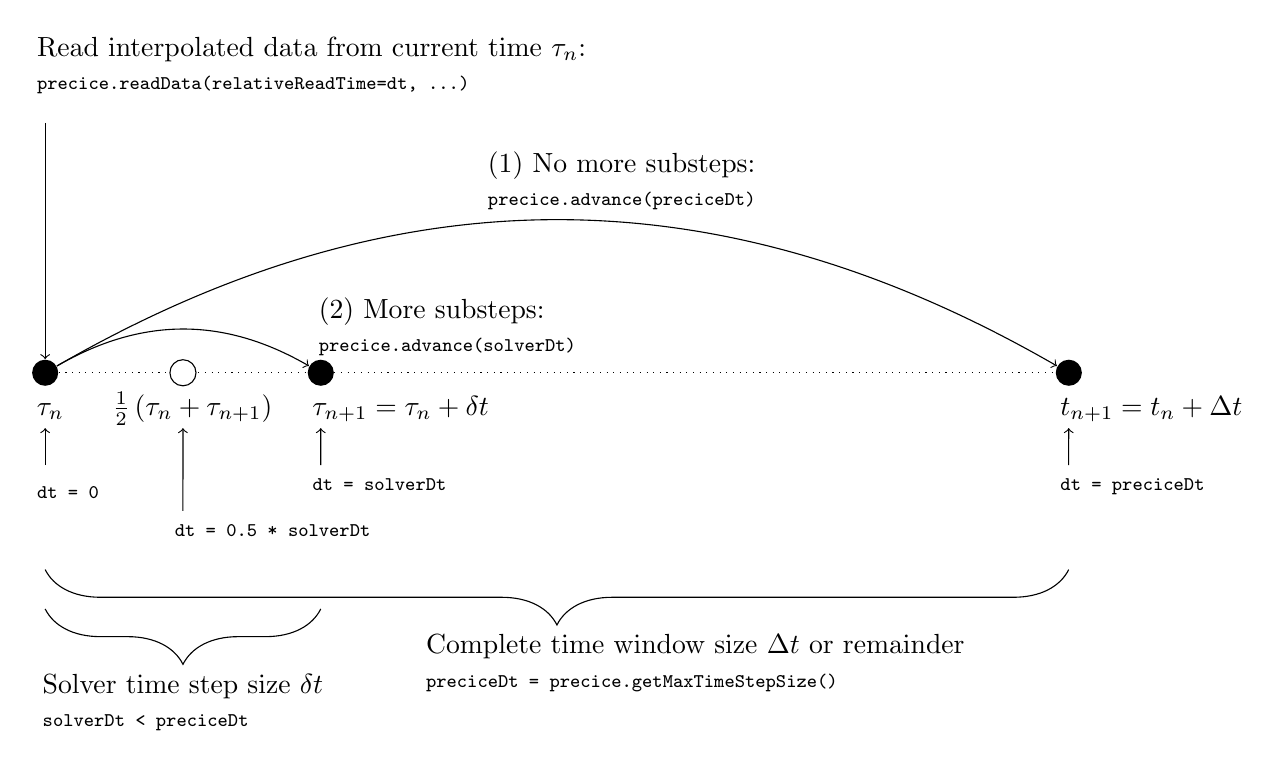
\begin{tikzpicture}[scale=10]
\node[circle, fill=black, label={[xshift=-1em]below right:$\vphantom{\frac{1}{2}}t_{n+1} = t_{n} + \Delta t$}](tnp1) at (1.3,0) {};
\node[circle, fill=black, label={[xshift=-1em]below right:$\vphantom{\frac{1}{2}}\tau_{n}$}](taun) at (0,0) {};
\node[circle, fill=black, label={[xshift=-1em]below right:$\vphantom{\frac{1}{2}}\tau_{n+1} = \tau_n + \delta t$}](taunp1) at (0.35,0) {};

\draw[->](taun) edge[out=30,in=150] node[above, align=left, anchor=south west,xshift=-1cm]{(1) No more substeps: \\ \scriptsize{\texttt{precice.advance(preciceDt)}}}(tnp1);
\draw[->](taun) edge[out=30,in=150] node[right, align=left, anchor=south west,pos=1]{(2) More substeps:\\  \scriptsize{\texttt{precice.advance(solverDt)}}} (taunp1);
\node[above = 3cm of taun, label={[xshift=-1em, align=left]above right:Read interpolated data from current time $\tau_n$:\\ \scriptsize\texttt{precice.readData(relativeReadTime=dt, ...)}}](tau) {};
\draw[->](tau) -- (taun);

\node[below = of taun, label={[xshift=-1em,yshift=0.1cm]below right:\scriptsize\texttt{dt = 0}}](rdt0) {};
\draw[->](rdt0) -- ($(taun)-(0,.2em)$);

\draw[dotted] (taun) -- (taunp1);
\draw[dotted] (taunp1) -- (tnp1);

\node[circle, draw=black, fill=white, label={[xshift=-3.25em]below right:$\frac{1}{2}\left(\tau_n + \tau_{n+1}\right)$}](subcyclingmid) at ($0.5*(taun) + 0.5*(taunp1)$) {};
\node[below = 4.5em of subcyclingmid, label={[xshift=-1em,yshift=0.2cm]below right:{\scriptsize\texttt{dt = 0.5 * solverDt}}}](rdtmid) {};
\draw[->](rdtmid) -- ($(subcyclingmid)-(0,.2em)$);

\node[below = of taunp1, label={[xshift=-1em,yshift=0.2cm]below right:\scriptsize\texttt{dt = solverDt}}](rdt1) {};
\draw[->](rdt1) -- ($(taunp1)-(0,.2em)$);

\node[below = of tnp1, label={[align=center,xshift=-1em,yshift=0.2cm]below right:\scriptsize\texttt{dt = preciceDt}}](rdtend) {};
\draw[->](rdtend) -- ($(tnp1)-(0,.2em)$);


\draw [decorate,decoration={brace,amplitude=2em,mirror}] ($(taun)-(0,.3)$) -- ($(taunp1)-(0,.3)$) node [black,midway,below,yshift=-2em, align=left] {Solver time step size $\delta t$\\ \scriptsize\texttt{solverDt < preciceDt} };

\draw [decorate,decoration={brace,amplitude=2em,mirror}] ($(taun)-(0,.25)$) -- ($(tnp1)-(0,.25)$) node [black,midway,below,yshift=-2em, xshift=5em, align=left] {Complete time window size $\Delta t$ or remainder\\ \scriptsize\texttt{preciceDt = precice.getMaxTimeStepSize()}};
\end{tikzpicture}

\end{document}

